%2011.4.3 ヤマサキ 振り子の問題に入るまでを結構いじりました。
%振り子の問題に入るまで この章は具体的な問題がないのと, 話が込み入ってくるのとを考えると, 「この章では何をやっているのか」が見失なわれがちではないかと思いました。
%そこで, この章での目標を「3次元空間における力学的エネルギー保存則を導くこと」とはっきり設定して, 話の順序を少し入れ替えてみました。
\chapter{力学的エネルギー保存則(2)}

第\ref{chapt:consenergy1}章では, 「力学的エネルギー保存則」が\textgt{直線上}(1次元)での質点の運動について, 
成り立つことを確かめた。本章では, この法則を, 3次元空間に拡張する。それによって, より多くの様々な現象を, 
「力学的エネルギー保存則」で解明できるのだ。

まず, これまで1次元の直線上での運動に限定して考えてきた「仕事」「ポテンシャルエネルギー」「運動エネルギー」
を, 3次元空間で再定義しよう。とりあえずいちばん簡単なのは「運動エネルギー」だ。\mv

\section{3次元空間における運動エネルギー}

第\ref{chapt:consenergy1}章を振り返ると, 質量$m$の質点が速度$v$で
直線的な運動(1次元の運動)をしているとき, その運動エネルギー$T(v)$は, 
\begin{eqnarray}
T(v)=\frac{1}{2}mv^2\label{eq:kineticEnergy_again}
\end{eqnarray}
と定義された(\eref{eq:kineticEnergy})。速度は本来, ベクトルなので, 
質点の運動が3次元的ならば, \eref{eq:kineticEnergy_again}の
$v^2$は速度ベクトル${\bf v}$によって, 
$|{\bf v}|^2$と置き換えたくなる。ここで, 
${\bf v}=(v_x, v_y, v_z)$とすると, 
$|{\bf v}|^2={\bf v}\bullet{\bf v}=v_x^2+v_y^2+v_z^2$
である。多くの教科書では, $|{\bf v}|^2$のことを単に${\bf v}^2$と書く慣習がある。
ここでもその慣習に習おう。すなわち, 
\begin{eqnarray} 
{\bf v}^2=v_x^2+v_y^2+v_z^2
\end{eqnarray} 
である(約束)。そこで, 3次元では, \eref{eq:kineticEnergy_again}のかわりに, 
\begin{eqnarray} 
T({\bf v})=\frac{1}{2}\,m{\bf v}^2=\frac{1}{2}\,m(v_x^2+v_y^2+v_z^2)\label{eq:kineticEnergy3D0}
\end{eqnarray}
を運動エネルギーの定義としよう。これは運動が1次元のときには, \eref{eq:kineticEnergy_again}に
帰着する。つまり, \eref{eq:kineticEnergy_again}を内包した定義になっている。\mv



\section{3次元空間における仕事}

次に, 仕事を3次元に拡張する。仕事とは, 「力と, その力が働く質点が"力と同じ向き"に動いた距離との掛け算」
であった。3次元空間でも, この定義を採用する:

ある質点にかかる力を${\bf F}$とし, その質点が動いた距離と
方向を表すベクトル(これを変位ベクトルという)を$\Delta{\bf r}$とする。${\bf F}$と$\Delta{\bf r}$のなす角を
$\theta$とすると, 「その力が働く質点が"力と同じ向き"に動いた距離」は, 
\begin{eqnarray} 
|\Delta{\bf r}|\cos\theta
\end{eqnarray} 
となる。従って, 仕事$W$は, 
\begin{eqnarray} 
W=|{\bf F}||\Delta{\bf r}|\cos\theta
\end{eqnarray} 
となる。ところが, 内積の定義から, これは
\begin{eqnarray} 
W={\bf F}\bullet\Delta{\bf r}\label{eq:work_Fdotdr}
\end{eqnarray} 
ということと同じである\footnote{\eref{eq:work_Fdotdr}の中の「$\bullet$」は, ベクトル
の内積を表す。内積とは何か, わからない人は, 
数学の教科書を参照せよ。}。\eref{eq:work_Fdotdr}は, \eref{eq:work}を3次元に拡張した
式でもある。

\begin{faq}{\small\textgt{ベクトルの内積なんてどうして
勉強するのかと思ってましたが, こういうことだったんですね。} ... 
他にも内積の用途はいろいろあります。}\end{faq}\mv

\eref{eq:work_Fdotdr}は, 質点が動く範囲で${\bf F}$が一定であるときにしか成り立たない。
一般には, ${\bf F}$は場所によって異なりうる。そこで, 
質点の移動の経路をたくさんの細かい区間に刻んで, 各区間では${\bf F}$がほとんど
一定であるとみなそう。つまり, \eref{eq:W_nF_nDx_n}から\eref{eq:work2}までと同じように考えればよい。

いま, 位置ベクトル${\bf r}_0$
の位置から位置ベクトル${\bf r}_n$の位置まで, 質点が力を受けて動くとしよう。この経路を細かく細かく刻み, 
途中の点の位置ベクトルを${\bf r}_1$, ${\bf r}_2$, ...とする。いま, $k$を1以上$n$以下の整数とし, 
${\bf r}_{k-1}$と${\bf r}_k$という隣接する2つの点を結ぶ変位ベクトルを
\begin{eqnarray}
\Delta {\bf r}_k={\bf r}_k-{\bf r}_{k-1}
\end{eqnarray}
とする。この2点の間で力は${\bf F}_k$でほぼ一定とする(図\ref{fig:work_3D})。\mv
\begin{figure}[h]
    \centering
    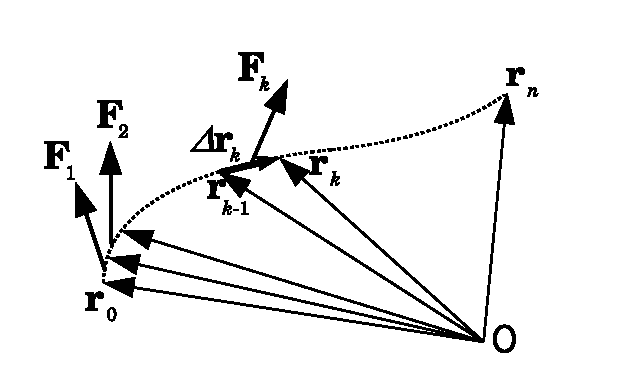
\includegraphics[width=7cm]{work_3D.eps}
    \caption{質点の動く経路を細かく分割する。}\label{fig:work_3D}
\end{figure}
この2点の間で力がなす仕事$\Delta W_k$は, 
\eref{eq:work_Fdotdr}より
$\Delta W_k\fallingdotseq{\bf F}_k\bullet\Delta {\bf r}_k$
となる。これを全区間について合計すれば, ${\bf r}_0$から${\bf r}_n$までの
移動でなされる仕事$W$になる:
\begin{eqnarray} 
W\fallingdotseq\sum_{k=1}^n \Delta W_k\fallingdotseq\sum_{k=1}^n {\bf F}_k\bullet\Delta {\bf r}_k
\end{eqnarray}
これは\eref{eq:one_step_before_work2}を3次元に拡張した式でもある。 
ここで刻みをどんどん小さくしていけば, 
\begin{eqnarray}
W=\lim_{\substack{n\rightarrow \infty\\\Delta {\bf r}_k\rightarrow 0}}\quad\sum_{k=1}^n{\bf F}_k\bullet\Delta {\bf r}_k
\end{eqnarray}
となる。これは積分の定義より($\Sigma$は$\int$になり, $\Delta$は$d$になる!), 
\begin{eqnarray} 
W=\int_{{\bf r}_0}^{{\bf r}} {\bf F}\bullet d{\bf r}
\end{eqnarray} 
となる(${\bf r}_n$を改めて${\bf r}$とおいた)。

\begin{faq}{\small\textgt{何ですかこの積分!? 
普通の積分は, $\int$なんちゃら$dx$とか$\int$なんちゃら$dt$みたいに, $d$が
つくのは$x$や$t$などです。でも, これは$d{\bf r}$って, ベクトルに
$d$がついてます。しかも内積!?} ... 
初めて見たらちょっとびっくりしますよね。でも, これはそんなに不思議なことではありません。
積分の定義を思い出して下さい。「関数と微小量の掛け算」が, ここでは
力(位置の関数で, ベクトル)と変位(位置の変化を表す微小量で, ベクトル)
の内積(掛け算をベクトルに拡張したもの)になっているだけです。}\end{faq}\mv

この式は\eref{eq:work2}を3次元に拡張した式だ。この積分は, 始点${\bf r}_0$と
終点${\bf r}$のみならず, 移動の経路にも依存するから, その経路を$\Gamma$と名づければ, 
以下のように言える: 経路$\Gamma$を移動する質点にかかる力${\bf F}$のなす仕事を, 
次式で定義する:
\begin{eqnarray}
W=\int_{\Gamma} {\bf F}\bullet d{\bf r}\label{eq:def_work_3D}
\end{eqnarray} 
ここで, ${\bf r}$は位置ベクトル。この式は, 最も一般的な仕事の定義式である。

ここで出てきた積分は, 君にとって目新しいものだろう。ここでは被積分関数も積分変数も
ベクトルであり, 「関数と微小量の掛け算」がここではベクトルの内積であり, 
しかも積分区間が「経路$\Gamma$」であるのだ。このように, ある経路に
沿って, ベクトルと微小ベクトルの内積を足し合わせるような積分を, 
\underline{線積分}\index{せんせきぶん@線積分}という。3次元では, 仕事は
線積分で定義されるのだ。\mv

\begin{q}\label{q:work_3D}
仕事を3次元空間で定義せよ。
\end{q}
\hv


\section{3次元空間におけるポテンシャルエネルギー}

次に, 「ポテンシャルエネルギー」の定義を3次元空間に拡張しよう。といっても, 
仕事の定義を上述のように改めること以外は, ポテンシャルエネルギーの定義は
1次元のときと同じだ。\eref{eq:potential}, つまり, 
\eref{eq:potential2}, \eref{eq:potential3}の位置$x$を
位置ベクトル${\bf r}$に置き換えたものが, 3次元空間における
ポテンシャルエネルギーだ。すなわち, ポテンシャルエネルギーを$U({\bf r})$とすると, 
\begin{eqnarray}
\text{定義1': }U({\bf r}):=-W({\bf r})\label{eq:3Dpotential}
\end{eqnarray}
ここで$W({\bf r})$は, 物体を基準点から点${\bf r}$まで運ぶときに, 
物体にかかっている保存力がなす仕事。
\begin{eqnarray}
\text{定義2': }U({\bf r}):=W'({\bf r})\label{eq:3Dpotential2}
\end{eqnarray}
ここで$W'({\bf r})$は, 物体を基準点から点${\bf r}$まで運ぶときに, 
かかっている保存力に逆らって誰かがなす仕事。
\begin{eqnarray}
\text{定義3': }U({\bf r}):=W''({\bf r})\label{eq:2Dpotential3}
\end{eqnarray}
ここで$W''({\bf r})$は, 物体を点${\bf r}$から基準点まで運ぶときに, 物体に
かかっている保存力がなす仕事。\\

無論, これらの3つの定義は互いに同値だ。力が保存力でなければ
ならない, ということに注意しよう。\mv

%
\begin{q}\label{q:3D_work_conservative}
物体が保存力${\bf F}$を受けて, ある点${\bf r}_0$から別の点${\bf r}_1$まで
移動するとき, ${\bf F}$がなす仕事$W_{01}$は, 
\begin{eqnarray}
W_{01}=U({\bf r}_0)-U({\bf r}_1)\label{3D_work_conservative}
\end{eqnarray}
であることを示せ。ここで$U$はポテンシャルエネルギーである。
\end{q}

%
\begin{q}\label{q:work_conservative_loop}
保存力が, 3次元空間の任意の閉曲線(始点と終点が一致する曲線)に沿ってなす仕事は, 必ず0になることを示せ。
\end{q}
\hv



\section{3次元空間における力学的エネルギー保存則}

役者は揃った。ではいよいよ, 力学的エネルギー保存則が3次元でも成り立つことを確認していこう。
1次元で力学的エネルギー保存則を導いたとき, \eref{eq:WandT00}から\eref{eq:WandT00s}に
かけて, 運動方程式を位置で積分した。3次元でも同じ事をやるのだ。まず, 運動方程式:
\begin{eqnarray}
{\bf F}=m\frac{d{\bf v}}{dt}\label{eq:3D_cons_F_ma}
\end{eqnarray}
を考える。${\bf F}$, ${\bf v}$, $m$, $t$はそれぞれ質点に働く力, 質点の速度, 質点の質量, 
そして時刻である。質点の位置ベクトルを${\bf r}(t)$とする。時刻$t$と, そこから
微小時間$dt$だけ経過した$t+dt$で, 質点は少し違う位置にいる(移動している)。その差, 
つまり変位を$d{\bf r}$と書こう。つまり, 
\begin{eqnarray}
d{\bf r}={\bf r}(t+dt)-{\bf r}(t)
\end{eqnarray}
である。この両辺を$dt$で割ったもの(つまり位置を時刻で微分したもの)
が速度${\bf v}$だ。つまり, ${\bf v}=d{\bf r}/dt$だ。従って, 次式が成り立つ:
\begin{eqnarray}
d{\bf r}={\bf v}dt\label{eq:3D_cons_dr_vdt}
\end{eqnarray}
\eref{eq:3D_cons_F_ma}に\eref{eq:3D_cons_dr_vdt}を辺々, 内積すると次式を得る:
\begin{eqnarray}
{\bf F}\bullet d{\bf r}=m\frac{d{\bf v}}{dt}\bullet {\bf v}dt\label{eq:3D_WandT000}
\end{eqnarray}
これはちょうど, \eref{eq:WandT000}を3次元に拡張した式だ。

ここで, 時刻$t_0$から$t_1$までの運動を考える。
${\bf r}_0={\bf r}(t_0)$, 
${\bf r}_1={\bf r}(t_1)$, 
${\bf v}_0={\bf v}(t_0)$, 
${\bf v}_1={\bf v}(t_1)$
とし, ${\bf r}_0$から${\bf r}_1$までの質点の運動の軌跡を$\Gamma$とする。
$\Gamma$をたくさんの短い区間に分割し, それぞれの区間で\eref{eq:3D_WandT000}
を考えて足し合わせる。つまり, 時刻$t_0$から$t_1$までの間で, 
\eref{eq:3D_WandT000}を積分すると, 
\begin{eqnarray}
\int_{\Gamma}{\bf F}\bullet d{\bf r}=\int_{t_0}^{t_1}m\frac{d{\bf v}}{dt}\bullet {\bf v}dt\label{eq:3D_WandT00s}
\end{eqnarray}
となる。左辺は\eref{eq:def_work_3D}の右辺
と同じ形になっている。つまり, 質点に働く力がなす仕事$W_{01}$である。

ここで, ${\bf v}=(v_x, v_y, v_z)$とすれば, 
\begin{eqnarray}
\frac{d{\bf v}}{dt}=\Bigl(\frac{dv_x}{dt}, \frac{dv_y}{dt}, \frac{dv_z}{dt}\Bigr)
\end{eqnarray}
である。これらを使って\eref{eq:3D_WandT00s}の右辺を成分で書くと, 次のようになる:
\begin{eqnarray}
&&\int_{t_0}^{t_1}m\Bigl(\frac{dv_x}{dt}, \frac{dv_y}{dt}, \frac{dv_z}{dt}\Bigr)\bullet(v_x, v_y, v_z)dt\\
&&=\int_{t_0}^{t_1}m\Bigl(v_x\frac{dv_x}{dt}+v_y\frac{dv_y}{dt}+v_z\frac{dv_z}{dt}\Bigr)dt\\
&&=\int_{t_0}^{t_1}mv_x\frac{dv_x}{dt}dt+\int_{t_0}^{t_1}mv_y\frac{dv_y}{dt}dt+\int_{t_0}^{t_1}mv_z\frac{dv_z}{dt}dt\nonumber\\
&&=\int_{v_x(t_0)}^{v_x(t_1)}mv_x\,dv_x+\int_{v_y(t_0)}^{v_y(t_1)}mv_y\,dv_y+\int_{v_z(t_0)}^{v_z(t_1)}mv_z\,dv_z\nonumber\\
&&=\Bigl[\frac{1}{2}m v_x^2\Bigr]_{v_x(t_0)}^{v_x(t_1)}+\Bigl[\frac{1}{2}m v_y^2\Bigr]_{v_y(t_0)}^{v_y(t_1)}+\Bigl[\frac{1}{2}m v_z^2\Bigr]_{v_z(t_0)}^{v_z(t_1)}\nonumber\\
&&=\frac{1}{2}m\bigl(v_x^2(t_1)+v_y^2(t_1)+v_z^2(t_1)\bigr)\nonumber\\
&&\,\,\,\,-\frac{1}{2}m\bigl(v_x^2(t_0)+v_y^2(t_0)+v_z^2(t_0)\bigr)\\
&&=\frac{1}{2}m{\bf v}_1^2-\frac{1}{2}m{\bf v}_0^2
\end{eqnarray}
となる。従って, \eref{eq:3D_WandT00s}は次式のようになる:
\begin{eqnarray}
W_{01}=\frac{1}{2}m{\bf v}_1^2-\frac{1}{2}m{\bf v}_0^2\label{eq:3DWandT0}
\end{eqnarray}
ここで\eref{eq:kineticEnergy3D0}を使うと, \eref{eq:3DWandT0}は
\begin{eqnarray}
W_{01}=T({\bf v}_1)-T({\bf v}_0)\label{eq:3D_WandT2}
\end{eqnarray}
となる。ここで, $T({\bf v})$は質点の運動エネルギーである。

\eref{eq:3D_WandT2}は, 1次元で導いた\eref{eq:WandT2}と同じ形の式だ。
つまり, 3次元の運動でも, 力がなした仕事は運動エネルギーの変化に等しい, 
ということが成り立つ。

ところで, \underline{力が保存力の場合は}, \eref{eq:3D_WandT2}の
左辺を\eref{3D_work_conservative}で書き換えると, 
\begin{eqnarray}
U({\bf r}_0)-U({\bf r}_1)=T({\bf v}_1)-T({\bf v}_0)\label{3D_work_conservative0}
\end{eqnarray}
となる。あるいは, 
\begin{eqnarray}
T({\bf v}_0)+U({\bf r}_0)=T({\bf v}_1)+U({\bf r}_1)\label{3D_work_conservative1}
\end{eqnarray}
となる。すなわち, 運動の最初(時刻$t_0$)と運動の最後(時刻$t_1$)で, 
「運動エネルギーとポテンシャルエネルギーの和」は等しいのだ。1次元のときと同様に, 
「運動エネルギーとポテンシャルエネルギーの和」のことを, 「力学的エネルギー」と
呼ぼう(定義)。すなわち, \eref{3D_work_conservative1}によって, 3次元における
力学的エネルギー保存則が確かめられた!\\

\begin{q}\label{q:consmom3D} 運動方程式から\eref{3D_work_conservative1}を導出せよ
(上の議論を整理・再現すればよい)。\end{q}


\begin{figure}[h]
    \centering
    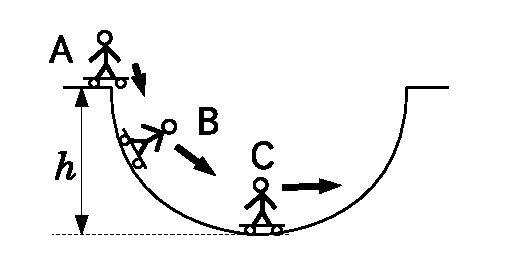
\includegraphics[width=7cm]{half_pipe.eps}
    \caption{スケートボードのハーフパイプ}\label{fig:half_pipe}
\end{figure}
\begin{q}\label{q:half_pipe}
スケートボードで, ハーフパイプを降りる人(スケートボードとあわせて質量$m$)の運動を考えよう(図\ref{fig:half_pipe})。
ハーフパイプの縁Aにいるときは速さ0である。そこから静かにハーフパイプの側面を降りはじめ, 
重力にまかせて加速しながら降りていき(点B), ハーフパイプの底(点C)に至る。点Cに至ったときは, 速さ$v$で水平方向に
動いている。ハーフパイプの底と縁の高度差は$h$であるとする。ただし摩擦や空気抵抗や車輪の回転に伴うエネルギーなどは無視する。
\begin{enumerate}
\item 重力加速度を$g$とする。次式を示せ:
\begin{eqnarray}\frac{1}{2}mv^2=mgh\end{eqnarray}
\item $h=5.0$~mのとき, $v$を求めよ。
\item ハーフパイプの断面が半円だとすると, 点Cでその人が受ける垂直抗力の大きさは重力の何倍か?
\end{enumerate}\end{q}

\section{振り子の運動}\index{ふりこ@振り子}

振り子の運動を考えてみよう。天井に固定された点Pから長さ$l$の糸が垂れており, 
その先に質量$m$の質点がついている(図\ref{fig:pendulum})。
質点が最も下に来たとき(糸が鉛直になったとき)の位置をOとする。糸をぴんと
張ったまま質点を少し持ち上げたときの
位置をQとする。Qから静かに質点を手放すと, 質点はP, O, Qを含む鉛直平面内で振動運動をする。

時刻$t$で質点は点X($t$)にあるとし, 角OPXをラジアンであらわしたものを$\theta$としよう。
当然, $\theta$は時間の関数だ。
以下, 糸の質量は0とする。空気抵抗は無視する。\mv
\begin{figure}[h]
    \centering
    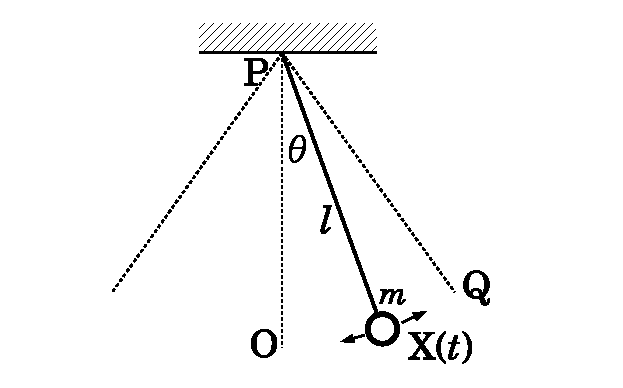
\includegraphics[width=7cm]{pendulum.eps}
    \caption{振り子}\label{fig:pendulum}
\end{figure}

\begin{q}\label{q:furiko_energy} この質点の運動について, \\
(1) 時刻$t$における質点の速度を${\bf v}(t)$とすると, 
\begin{eqnarray} 
|{\bf v}(t)|=\Bigl|l\frac{d\theta}{dt}\Bigr|
\end{eqnarray} 
であることを示せ。{\small ヒント:$t$から$t+dt$の間に$X$が移動するのは, 扇形の
弧の部分である。その弧の長さ(つまり移動距離)は, 
「半径」かける「角度の変化」であり, 「角度の変化」
は$\theta(t+dt)-\theta(t)$である。また, 速度の絶対値(つまり速さ)とは, 
$t$から$t+dt$の間に$X$が移動した距離を時間間隔$dt$で割ったものだ。}\\
(2) 時刻$t$における質点の運動エネルギー$T$とポテンシャルエネルギー$U$は, それぞれ
次のようになることを示せ:
\begin{eqnarray} 
T&=&\frac{1}{2}m l^2\Bigl(\frac{d\theta}{dt}\Bigr)^2\\
U&=&mgl(1-\cos \theta)
\end{eqnarray} 
ただし, 質点が点Oにあるとき$U=0$と定める。\\
(3) 働く力は重力と張力だけだが, 重力は保存力であり, 張力は仕事をしない
(移動方向と力の方向が直交しているので)。従って力学的エネルギー保存則が成り立つ。
すなわち, $T+U$は時刻$t$によらず一定である。従って, 
$T+U$を$t$で微分すると, 0にならねばならない。このことから, 次式を導け:
\begin{eqnarray} 
ml^2\frac{d\theta}{dt}\frac{d^2\theta}{dt^2}+mgl\sin\theta\frac{d\theta}{dt}=0
\end{eqnarray} 
(4) その結果, 次式(振り子の運動をあらわす微分方程式)を得ることを示せ:
\begin{eqnarray} 
\frac{d^2\theta}{dt^2}=-\frac{g}{l}\sin\theta\label{eq:furiko_equation}
\end{eqnarray} 
(5) $\theta$が0に近い場合, 振り子の運動方程式は, 近似的に次のようになることを示せ:
\begin{eqnarray} 
\frac{d^2\theta}{dt^2}=-\frac{g}{l}\theta\label{eq:furiko_energy5}
\end{eqnarray} 
この近似式が成り立つとして, 以下の小問に答えよ:\\
(6) $\omega=\sqrt{g/l}$とすると\eref{eq:furiko_energy5}は次式になることを示せ
(これは関数$\theta(t)$に関する微分方程式):
\begin{eqnarray} 
\frac{d^2\theta}{dt^2}=-\omega^2\theta\label{eq:furiko_energy6}
\end{eqnarray} 
(7) $\theta(t)=\theta_0 \cos\omega t$は上の微分方程式の解であることを示せ。ただし$\theta_0$は定数とする。\\
(8) 振り子の周期$\tau$を, $g$と$l$であらわせ\footnote{普通は周期は$T$で表す慣習が多いが, ここでは$T$は運動エネルギーの記号に使っているので, 周期は$\tau$(ギリシア文字のタウ)を使う。}。\\
(9) $l=1.0$~mのとき, 振り子の振動の角速度と周期は?\\
(10) $l$を何倍にすれば振り子の周期は半分になるか?
\end{q}


\begin{q}\label{q:furiko_period}
前問で見たように, \underline{振幅が十分に小さいとき} \underline{に限れば}
(すなわち$\theta$が0に近ければ), 振り子の周期は糸の長さ$l$と重力加速度$g$
だけで決まってしまい, 質点の質量$m$や, 振れ幅$\theta_0$などには依らない。これは, 振り子の
重要な性質である(これを「振り子の等時性という」\index{とうじせい@等時性})。
\begin{enumerate}
\item これを利用して, 重力加速度$g$を測定する。つまり, 長さ$l$の糸の先に適当な重り
をつけて振動させ, その周期$\tau$を測ったとする。では, $l$と$\tau$から$g$を求める式は? 
\item 月面では, 地球上に比べて振り子の周期は何倍になるか? 
\end{enumerate}
\end{q}

\begin{q} 2つの互いに同仕様の振り子時計がある。これらの時刻を互いに合わせた後, 
東京(重力加速度9.798~m~s$^{-2}$)と札幌(重力加速度9.805~m~s$^{-2}$)
のそれぞれに置いた。1日たつと, 札幌の時計は東京の時計より何秒, 進んでいる
(もしくは遅れている)か?\end{q}
\mv

\begin{faq}{\small\textgt{振り子といえばフーコーですね。振り子で地球の自転を証明したんですよね} ... 
そうです。自転によって生じる「コリオリ力」という見かけの力を実証しました。}\end{faq}\mv
\hv

\section{ポテンシャルエネルギーと力の関係}

{\small (本節は後の話に関係しないので読み飛ばしてもよい。
秋学期に電磁気学を学ぶ時に復習すると役立つだろう。)\\}

さて, 力学的エネルギー保存則の話から少し外れるが, ここで力とポテンシャルエネルギーの関係をもう少し深くみておこう。
いま, 符号を無視しておおまかに言えば, 力の(線)積分がポテンシャルエネルギーを与えるわけだから, 積分と微分は
互いに逆の操作であることを考えれば, ポテンシャルエネルギーの微分が力を与えるのではないだろうか? 
実は, この発想は正しい。以下にそれを説明しよう:

いま, ある質点に働く力が保存力であり, しかも場所だけによって一意的に定まり, 時刻や速度など
には陽に依存しない\footnote{この「陽に」(explicit)という言葉は科学ではよく使う。「あからさまに」
とか「直接的に」という意味。今の場合は, 時間と共に場所が変われば力も変わるかもしれないが, 
それは場所が変わったからであり, 時間の変化が直接的に力を変えたわけではない, ということ。}
としよう。

とりあえず, 簡単のため, 物体の移動は直線上($x軸$の上)に制限され, 働く力もその直線に沿った方向に
限定されるとしよう。物体が位置$x_0$から$x_1$まで動くときに, 力$F$がなす仕事$W_{01}$は, 
\eref{eq:W01U1U0}より, 
\begin{eqnarray}
W_{01}=-U(x_1)+U(x_0)
\end{eqnarray}
である($U$はポテンシャルエネルギー)。ここで, $x_0$を$x$とし, $x_1$を$x$から非常に近い位置$x+dx$とすると($dx$は0に近い量), 
\begin{eqnarray}
W_{01}=-U(x+dx)+U(x)\label{eq:W01UxdxUx}
\end{eqnarray}
となる。ところで, 仕事の定義から, $W_{01}$は
$W_{01}=F\,dx$である。これらから, 
$F\,dx=-U(x+dx)+U(x)$
となる。両辺を$dx$で割って, 
\begin{eqnarray}
F=-\frac{U(x+dx)-U(x)}{dx}
\end{eqnarray}
ここで$dx$が十分に0に近いことを思い出せば, 
\begin{itembox}{ポテンシャルエネルギーと力の関係(1次元)}
\begin{eqnarray}
F=-\frac{dU}{dx}
\end{eqnarray}
\end{itembox}
である。つまり, 力は, ポテンシャルエネルギーを微分してマイナスをつけたものに等しい。\mv

この話は3次元空間に拡張できる。物体が力${\bf F}$を受けながら位置${\bf r}$から, 
わずかだけ離れた位置${\bf r}+d{\bf r}$に移動することを考える。
\begin{eqnarray}
d{\bf r}=(dx,\, dy,\, dz)
\end{eqnarray}
は十分に小さいベクトルである。
すると, 力がなす仕事$W$は, \eref{eq:W01UxdxUx}と同じように考えれば, 
\begin{eqnarray}
W=-U({\bf r}+d{\bf r})+U({\bf r})\label{eq:dW3D}
\end{eqnarray}
である($U$はポテンシャルエネルギー)。ここで全微分\footnote{数学の教科書を参照。}を使うと, 
$U({\bf r}+d{\bf r})=U(x+dx, y+dy, z+dz)$
\begin{eqnarray}
&=&U(x, y, z)+\frac{\partial U}{\partial x}dx+\frac{\partial U}{\partial y}dy+\frac{\partial U}{\partial z}dz\nonumber\\
&=&U({\bf r})+\frac{\partial U}{\partial x}dx+\frac{\partial U}{\partial y}dy+\frac{\partial U}{\partial z}dz\,\,\,\,\,\,\,\,\,\,\,\,\,\,\,\,\,\,\,\,\,\,\,
\end{eqnarray}
である。これを\eref{eq:dW3D}に代入すると次式になる:
\begin{eqnarray}
W&=&-U({\bf r})-\frac{\partial U}{\partial x}dx-\frac{\partial U}{\partial y}dy-\frac{\partial U}{\partial z}dz+U({\bf r})\nonumber\\
 &=&-\frac{\partial U}{\partial x}dx-\frac{\partial U}{\partial y}dy-\frac{\partial U}{\partial z}dz\nonumber\\
 &=&-\Bigl(\frac{\partial U}{\partial x}, \frac{\partial U}{\partial y}, \frac{\partial U}{\partial z}\Bigr)\bullet(dx, dy, dz)\nonumber\\
 &=&-\Bigl(\frac{\partial U}{\partial x}, \frac{\partial U}{\partial y}, \frac{\partial U}{\partial z}\Bigr)\bullet d{\bf r}
\end{eqnarray}
一方, 仕事の定義から$W$は$W={\bf F}\bullet d{\bf r}$なので, 
\begin{eqnarray} 
{\bf F}\bullet d{\bf r}=-\Bigl(\frac{\partial U}{\partial x}, \frac{\partial U}{\partial y}, \frac{\partial U}{\partial z}\Bigr)\bullet d{\bf r}\label{eq:Fdr_gradUdr}
\end{eqnarray} 
である。$dx, dy, dz$は0に近い任意の量なので, 上の式が成り立つには, 
\begin{itembox}{ポテンシャルエネルギーと力の関係(3次元)}
\begin{eqnarray} 
{\bf F}=-\Bigl(\frac{\partial U}{\partial x}, \frac{\partial U}{\partial y}, \frac{\partial U}{\partial z}\Bigr)\label{eq:F_gradU}
\end{eqnarray} 
\end{itembox}
でなければならない\footnote{
${\bf F}=(F_x, F_y, F_z)$とする。\eref{eq:Fdr_gradUdr}で$dx\ne0$として$dy=dz=0$とすると, 
\begin{eqnarray*}F_x\,dx=-\frac{\partial U}{\partial x}\,dx,\,\,\,\,\,\,\,\text{したがって, }\,\,\,F_x=-\frac{\partial U}{\partial x}\end{eqnarray*}
を得る。$dy\ne0$で$dx=dz=0$の場合や, $dz\ne0$で$dx=dy=0$の場合も同様に考えれば, 
\begin{eqnarray*}F_y=-\frac{\partial U}{\partial y},\,\,\,\,F_z=-\frac{\partial U}{\partial z}\end{eqnarray*}
を得る。したがって\eref{eq:F_gradU}が成り立つ。}。ここで, "grad"という記号を, 
\begin{eqnarray}
\grad U=\Bigl(\frac{\partial U}{\partial x}, \frac{\partial U}{\partial y}, \frac{\partial U}{\partial z}\Bigr)
\end{eqnarray}
と定義する\footnote{このgradとは, "gradient"の略であり, 日本語では「勾配」と言う。
その意味は, いずれ基礎数学や秋学期の物理学で学ぶだろう。}。この記号を使うと, 
\eref{eq:F_gradU}は次式のように書ける:
\begin{eqnarray} 
{\bf F}=-\grad U\label{eq:F_gradU2}
\end{eqnarray} 
\mv

\begin{exq} アインシュタインの相対性理論によると, 重力によるポテンシャル
エネルギーが高い位置ほど時間は速く進む(とても不思議!)。すなわち, ある
2つの位置A, Bがあって, 重力によるポテンシャルエネルギーが, 位置Bでは
位置Aよりも$m\phi$だけ高いとし($m$は質点の質量), 位置Aに置かれた時計が
時間$T$だけ進む場合, 位置Bに置かれた時計は, 以下のぶんだけ進む。
\begin{eqnarray}
T\Bigl(1+\frac{\phi}{c^2}\Bigr)
\end{eqnarray}
ここで, $c=299792458$~m/sは光の速さである。
以後, 地球の半径を$R=6400$~kmとする。\\
(1) GPS衛星は地表から約20,000~kmの高さを飛んでいる。地上の時計が
1秒進む間に, GPS衛星に搭載された時計は, 1秒よりどれだけ多くの時間を進むか? 
(他の要因のために, 実際に起きるのは, ここで計算される値よりも, 若干小さい値である)\\
(2) 高精度の時計が2つあれば, これらの時計が示す時刻の差から, これらの時計の
置かれた高さの差がわかる。つまり, 時計を高度計として使うことができるだろう。
ところで, 東大の香取秀俊博士が開発した「光格子時計」は, 300億年に1秒しか狂わない
という, 世界的にもブッチギリな高精度を持つ。この時計を高度計として使う場合, 
地表付近(海面から高さ±数kmの範囲)では, どのくらいの誤差で高度を計測できるか?
\end{exq}

なお, この「高度計」が素晴らしいのは, GPSのような衛星からの電波が入ってこない水中や
地下, 屋内などでも原理的には利用可能ということである。\\

\section{解答}
% 仕事を3次元空間で定義せよ。
%\noindent{\textbf{答}}\ref{q:work_3D} 質点を経路$\Gamma$に沿って移動するとき, 
%各位置で質点にかかる力を${\bf F}$とすると, その経路に沿って${\bf F}$が質点に
%対してなした仕事$W$は, 
%\begin{eqnarray*} 
%W=\int_{\Gamma} {\bf F}\bullet d{\bf r}
%\end{eqnarray*}
%である。\mv
\noindent{\textbf{答}}\ref{q:work_3D} 略。\mv

%
\begin{figure}[h]
    \centering
    \includegraphics[width=5.0cm]{cons_force_3D.eps}
    \caption{問\ref{q:3D_work_conservative}の仕事の経路。}\label{fig:cons_force_3D}
\end{figure}
\noindent{\textbf{答}}\ref{q:3D_work_conservative}
物体を基準点から点${\bf r}_0$まで運ぶときに保存力${\bf F}$
がなす仕事を$W({\bf r}_0)$とすると, 定義から, 
\begin{eqnarray}
U({\bf r}_0)=-W({\bf r}_0)\label{q:3D_work_conservative_ans1}
\end{eqnarray}
である。同様に, 物体を基準点から点${\bf r}_1$まで運ぶときに保存力${\bf F}$
がなす仕事を$W({\bf r}_1)$とすると, 
\begin{eqnarray}
U({\bf r}_1)=-W({\bf r}_1)\label{q:3D_work_conservative_ans2}
\end{eqnarray}
である。ここで, 基準点から点${\bf r}_1$へ物体を運ぶときの経路を, 点${\bf r}_0$を
経由するようにとれば(図\ref{fig:cons_force_3D}), 保存力ゆえに仕事は経路によらず一定なので, 
$W({\bf r}_1)=W({\bf r}_0)+W_{01}$
となる。ここで$W_{01}$は物体を点${\bf r}_0$から点${\bf r}_1$に運ぶときの仕事。
この式の$W({\bf r}_0), W({\bf r}_1)$を, 
\eref{q:3D_work_conservative_ans1}, \eref{q:3D_work_conservative_ans2}を
使って置き換えると, 
$-U({\bf r}_1)=-U({\bf r}_0)+W_{01}$
となる。従って, 
$U({\bf r}_0)-U({\bf r}_1)=W_{01}$。
\mv

% 保存力が, 3次元空間の任意の閉曲線に沿ってなす仕事は, 必ず0に
\noindent{\textbf{答}}\ref{q:work_conservative_loop}
閉曲線$\Gamma$に沿う移動によってなす仕事を$W$とする。
移動の開始点を${\bf r}_0$とすると, 移動の終了点も${\bf r}_0$である。保存力だから, 
\eref{3D_work_conservative}で, ${\bf r}_1={\bf r}_0$, $W_{01}=W$として, 
$W=U({\bf r}_0)-U({\bf r}_0)$となる。右辺は0だから, 結局, $W=0$となる。\mv


\noindent{\textbf{答}}\ref{q:half_pipe} 
(1) 点Cをポテンシャルエネルギーの基準点とする。点Aでは, 運動エネルギーは0, 
ポテンシャルエネルギーは$mgh$である。従って力学的エネルギーは$mgh$となる。
点Cでは, 運動エネルギーは$mv^2/2$, ポテンシャルエネルギーは0である。従って力学的エネルギーは$mv^2/2$となる。
働く力は重力と垂直抗力だけだが, 重力は保存力であり, 垂直抗力は仕事をしない(移動方向と力の方向が直交しているので)。
従って力学的エネルギー保存則が成り立つ。すなわち, 点Aと点Cで力学的エネルギーは等しいことから, 与式を得る。\\
(2) 前小問より,
\begin{eqnarray*}
v=\sqrt{2gh}=\sqrt{2\times9.8\text{ m s}^{-2}\times5\text{ m}}=9.9\text{ m s}^{-1}
\end{eqnarray*}
(3) 半円形ハーフパイプの高さが$h$なのだから, この円の半径は$h$である。
\eref{eq:mvsqovr}より, C点では人は円の中心に向かって(つまり上向きに), 
$mv^2/h$という合力を受けるはず。
一方, 垂直抗力を$N$とする。人には下向きに$mg$という重力も働くから, 
上向きの力は, 垂直抗力と重力の合力であり, その大きさは$N-mg$である。従って, 
$N-mg=mv^2/h$である。従って, 
\begin{eqnarray}N=\frac{mv^2}{h}+mg\end{eqnarray}
である。小問(1)より$mv^2=2mgh$だから, 
\begin{eqnarray}N=2mg+mg=3mg\end{eqnarray}
となる。よって垂直抗力は, 半径$h$によらず, 重力の3倍。だからハーフパイプ走者は
重力の3倍の力に耐える頑丈な肉体を持っていなければならない。
\mv

% 天井に固定された点Pから長さ$l$の糸が垂れており, その先に
\noindent{\textbf{答}}\ref{q:furiko_energy} 
(1) $t$から$t+dt$の間に$X$が移動する距離は, \\
$l|\theta(t+dt)-\theta(t)|$である。微分の定義から, 
これは$l|\theta'dt|$に等しい。これを$dt$で割ったものが速度の大きさになる。したがって与式が成り立つ。
(2) 略($T=mv^2/2$の$v$に前小問の結果を代入すると, 運動エネルギー$T$の与式を得る。また, Oに比べてX
は$l(1-\cos\theta)$だけ高い位置にある。従って, 重力によるポテンシャルエネルギー$U$の与式を得る。)
(3), (4) 略。
(5) 略。($\sin \theta \fallingdotseq \theta$とすればよい)
(6) 略。
(7) 略(\eref{eq:furiko_energy6}の左辺と右辺に代入して, それらが等しくなることを示せばよい)。
(8) $\tau=2\pi/\omega$より(\eref{eq:vib_period}) 参照), 
\begin{eqnarray}\tau=2\pi\sqrt{l/g}\label{eq:furiko_energy_ans5}\end{eqnarray}
(9) 角速度は, $\omega=\sqrt{g/l}=\sqrt{9.8\text{ m s}^{-2}/(1.0\text{ m})}=3.1\text{ s}^{-1}$。周期は(計算略), $\tau=2\pi/\omega=2.0$ s。\\
(10) \eref{eq:furiko_energy_ans5}より, $\tau$は$\sqrt{l}$に比例するから, $\tau$を半分にするには, $\sqrt{l}$を半分にすればよい。従って$l$を1/4倍にすればよい。
\mv

% 前問で見たように, 振幅が十分に小さければ, 振り子の周期は
\noindent{\textbf{答}}\ref{q:furiko_period}
(1) \eref{eq:furiko_energy_ans5}を変形して$g=$の式にすると, 
$g=4\pi^2l/\tau^2$。
(2) 月面では重力加速度が地表の1/6倍になる。\eref{eq:furiko_energy_ans5}より, 
$\tau$は$1/\sqrt{g}$に比例するから, $g$が1/6倍になると$\tau$は$\sqrt{6}=2.4$倍(ゆっくり振動)。
\mv


\begin{faq}{\small\textgt{ポテンシャルエネルギーは, 力学的エネルギー保存則
を見やすくするために定義されたもの, と考えてよいのですか?} ... 
それだけではありません。まず, 力はベクトルだけどポテンシャルエネルギーはスカラーなので, 
力を直接考えるよりも, 数学的に取扱いがシンプルで楽になります。また, 量子力学では力よりも
ポテンシャルエネルギーの方が直接的に重要な働きをします。}\end{faq}

\begin{faq}{\small\textgt{力学的エネルギー保存則と
エネルギー保存則は違うんですね?} ... 違うというより, 
前者は後者の一種(特別なケース)ですね。}\end{faq}

\begin{faq}{\small\textgt{「保存力は径路に依存しない」というフレーズが頭にしっくりこない。} ... 
ちょっと省略しすぎですね。「保存力がなす仕事は, 径路によらず, 始点と終点だけで
決まる」というのが正しい表現です。例え話でいうと, 山を登るのに, きつい勾配の坂を
まっすぐ登るのと, ジグザグになった緩やかな道を登るのとでは, 全体の仕事(力かける距離)
は同じということです。きつい道では大きな力が(移動方向に)かかるけど, そのぶん
短くてすみます。}\end{faq}

\section*{コラム: ベクトルは太字, スカラーは細字なのはなぜか?}

{\small 「ベクトルは太字で書く」が, ちゃんとできない人が多い。そもそもなぜベクトルは特別な
書き方(太字で書く)をするのだろう?それは, スカラーとベクトルは, 本質的に違う量
であり, 計算ルールも異なるからだ。

例えば「スカラーでの割り算」は(0で割る以外は)許されるが, 「ベクトルでの割り算」は
許されない。スカラー同士やベクトル同士は足せるが, スカラーとベクトルは足せない。
スカラーとベクトルの大小関係は比べられないし, スカラーとベクトルが等号で結ばれる
こともない。それらの「ルール破り」を防ぐための「要注意記号」として, ベクトルを太字や
上付き矢印で書くのだ。

ベクトルは太字という慣習を守らない人は, そもそも何がベクトルで何がスカラーかを
わかっていない可能性がある。それはかなりヤバイ。ベクトルを太字で書かないと減点されるのは, 
「わかってる風を装っているだけで, 実はわかっていない」のではないかと思われているのだ。
逆に言えば, 「自分はどれがベクトルでどれがスカラーなのかちゃんとわかってるぜ!」
ということをアピールするために, ベクトルを太字で書くのだ。

ところが, ひとつの直線上に限定された現象(直線運動)では, ベクトルとスカラーを
区別する必要はないので, 本来ベクトルである量もスカラーとして扱い, 
細字で書く。このような場合も, 力や速度や加速度には向きがあるが, 
それは符号(正か負か)で表現できるので, スカラーで十分であり, 
わざわざベクトルとして扱う必要は無い。ベクトルとして扱っても, 
数値で表現するときは, ひとつの数値(成分)しかない。

数学や物理では, 「区別すべきものは区別せねばならないが, 区別する必要のない
ものは, 理由もないのに区別したりしてはいけない」という
慣習がある(例外もあるが)。これに照らせば, 直線上に限定されることが最初から
わかっている運動では$F=ma$のように書いてよいし, むしろそう書かねばならない
($F, m, a$は力, 質量, 加速度)。この場合は$F$や$a$はスカラーと
同様に扱うことができ, $m=F/a$と書けるからでもある($a\neq 0$の場合)。\\}


\section*{コラム: 問題を解くコツ}

{\small 物理学の問題を解くには, いくつかのコツがある。\\

1. 値の代入は最後にやる!

既に述べたが, 答を数値で求める問題も, できるだけぎりぎりまで, 数値ではなく文字の式変形で攻めよう。そして, 求めたい量を既知の量で表す式が求まった段階で, 既知の量の数値を代入して一気にまとめて数値計算をするのである。最初や途中から数値を代入してしまうと, 式変形と数値計算が混在してしまい, ミスを起こしやすく, また, ミスの発見がやりにくくなる。一方, 最後にまとめて計算すれば, 約分の組み合わせがたくさんできるので, 計算が効率よく, 正確にできる。\\

2. ベクトルかスカラーかを考える。

今扱っている量がベクトル(向きを持つ量)なのかスカラー(向きは持たず, 大きさだけを持つ量)なのかを意識しよう。速度, 加速度, 力, 運動量はベクトル。エネルギー, 仕事, 質量はスカラー。ベクトル=スカラーみたいな等式(方程式)は絶対に成り立たない。そんな変な式を立てていないかチェックしよう。そのためにも, ベクトルは太字で書く, ということを徹底しよう。\\

3. 次元をチェック!

式変形の途中や最終結果の次元をチェックしよう。例えば運動方程式を解いて, 質点の速度$v$に関する式を得たら, それが速度の次元を持っているかをチェックする。$v=\exp(-\alpha t/m)-mg$のような式を見たら, 一瞬で「これは違う!」と気づかねばならない(expは必ず無次元である...わからない人は「大学1年生のための数学入門」を見よう!)。次元をチェックしていれば, 単位を忘れる, ということはありえない。\\

4. 初期条件をチェック!

運動方程式を解く場合は, たいてい, 初期条件が与えられている。式変形の最後に得た式に, $t=0$を入れてみよう。それが初期条件が満たすかどうかをチェックしよう。\\

5. $t\rightarrow\infty$をチェック!

与えられた問題は, 時間が十分たてばどうなるかが常識的にわかることがある。例えば, 摩擦を受けて運動する物体は, いずれ止まったり, 一定速度に落ち着いたりすることが多い。運動方程式を解いて得た式で時刻$t$を$\infty$にしてみて, 実際にそうなるかどうかを確認しよう。\\

6. $x=0$や$t=0$のまわりで線形近似!

方程式を解いて得た式について, 0のまわりで線形近似してみよう。それは多くの場合, 得た式よりもシンプルになり, 直感的に解釈しやすい。例えば空気抵抗つきの自由落下の問題では, $t=0$のまわりでの線形近似は$v=-gt$のように簡単な式になる。それが君の物理的直感に整合するかを考えよう。\\

7. 保存則をチェック!

物理は, 運動方程式を解くのが正攻法だが, それを迂回するのが「保存則」である。条件設定によって, 保存する量とそうでない量がある。保存量があれば, それに着目して問題を考えるとシンプルに解けることが多い。運動方程式を立てたり解いたりする前に, 保存則が使えないかを考えよう。}
